Voici le diagramme représentant l'architecture globale de l'application :

\begin{figure}[H]
    \centering
    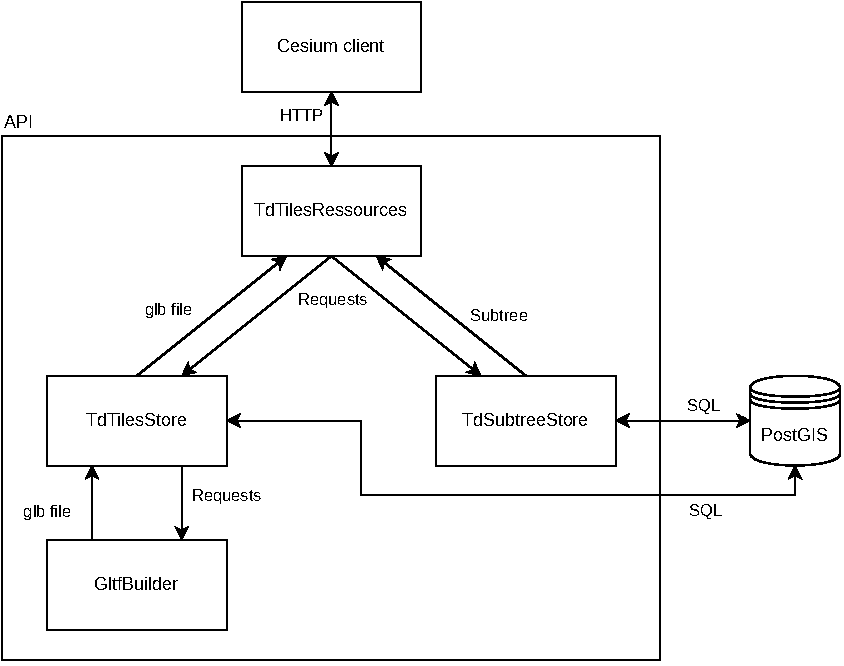
\includegraphics[width=1\textwidth]{assets/figures/architecture.drawio.pdf}
    \caption{Calcul du SSE \cite{3d-tiles-specification}}
    \label{fig:lods-colors}
\end{figure}

\newpage

Le client Cesium va en premier lieu demander les Subtrees à l'API afin qu'il puisse savoir quelles tuiles afficher. \texttt{TdTilesRessources} va transmettre cette requête à \texttt{TdSubtreeStore} qui va se charger de récupérer le Subtree dans la base de donnée si il existe ou sinon d'en créer un, de mettre à jour la base de donnée et de le retourner. Une fois que le client Cesium a reçu le Subtree, il va ensuite demander les Subtrees si il y en a et les contenus des tuiles affichables. Lorsque \texttt{TdTilesRessources} reçoit une demande de contenu d'une tuile, ell va transmettre cette demande à \texttt{TdTileStore} qui va se charger de récupérer le contenu de la tuile dans la base de donnée si il existe ou sinon de passer la demande à \texttt{GltfBuilder}. Ce dernier va générer le contenu de la tuile et le stocker dans la base de donnée avant de le retourner.